% Section 2: General-Form Prisoners' Dilemma Repeated
%-------------------------------------------------------------------------------

\begin{frame}{General Prisoners' Dilemma}
  \begin{table}[!h]
    \centering
    \begin{tabular}{*{4}{c|}}
      \multicolumn{2}{c}{} & \multicolumn{2}{c}{Column} \\ \cline{3-4}
      \multicolumn{1}{c}{} &         & Defect  & Cooperate \\ \cline{2-4}
      \multirow{2}*{Row} &    Defect & $D$,$D$ & $H$,$L$   \\ \cline{2-4}
                         & Cooperate & $L$,$H$ & $C$,$C$   \\ \cline{2-4} 
    \end{tabular} 
  \end{table} 

  What ordering of payoffs $D$, $H$, $L$, and $C$ make this a \textbf{Prisoners' Dilemma}? 
  \begin{enumerate}[label=\textbf{\alph*)}]
    \item $C > D > H > L$ 
    \item $H > D > C > L$ 
    \item $H > C > D > L$ 
    \item $C > H > L > D$
  \end{enumerate}
\end{frame}

\begin{frame}{General Prisoners' Dilemma}
  A single-stage prisoners' dilemma in extensive form:
  \usetikzlibrary{calc} 
  \begin{center}
  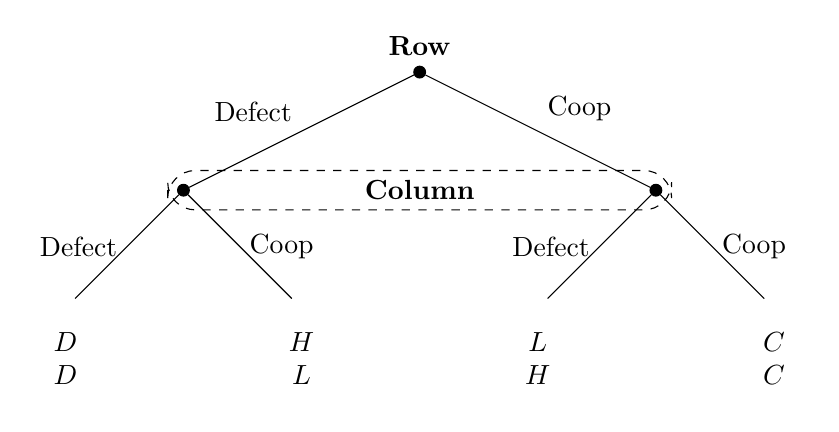
\begin{tikzpicture}
    \tikzstyle{solid node}=[circle,draw,inner sep=1.5,fill=black]
    \tikzstyle{level 1}=[level distance=15mm,sibling distance=6cm]
    \tikzstyle{level 2}=[level distance=15mm,sibling distance=3cm]
    \node(0)[solid node,label=above:{\textbf{Row}}]{}
        child{node(1)[solid node,label=above left:{}]{}
            child{node[label=below:{\begin{tabular}{c}
                    $D$ \\
                    $D$
                \end{tabular}}]{} edge from parent node[left]{Defect}}
            child{node[label=below:{\begin{tabular}{c}
                    $H$ \\
                    $L$
                \end{tabular}}]{} edge from parent node[right]{Coop}}
            edge from parent node[above left]{Defect}
        }
        child{node(2)[solid node,label=above right:{}]{}
            child{node[label=below:{\begin{tabular}{c}
                    $L$ \\
                    $H$
                \end{tabular}}]{} edge from parent node[left]{Defect}}
            child{node[label=below:{\begin{tabular}{c}
                    $C$ \\
                    $C$
                \end{tabular}}]{} edge from parent node[right]{Coop}}
            edge from parent node[above right]{Coop}
        };
    \draw[dashed,rounded corners=10]($(1) + (-.2,.25)$)rectangle($(2) +(.2,-.25)$);
    \node at($(1)!.5!(2)$){\textbf{Column}};
  \end{tikzpicture}
  \end{center}
\end{frame}

\begin{frame}{General Prisoners' Dilemma}
  A \textbf{two-stage} prisoners' dilemma in mixed extensive form:
  \usetikzlibrary{calc} 
  \begin{center}
    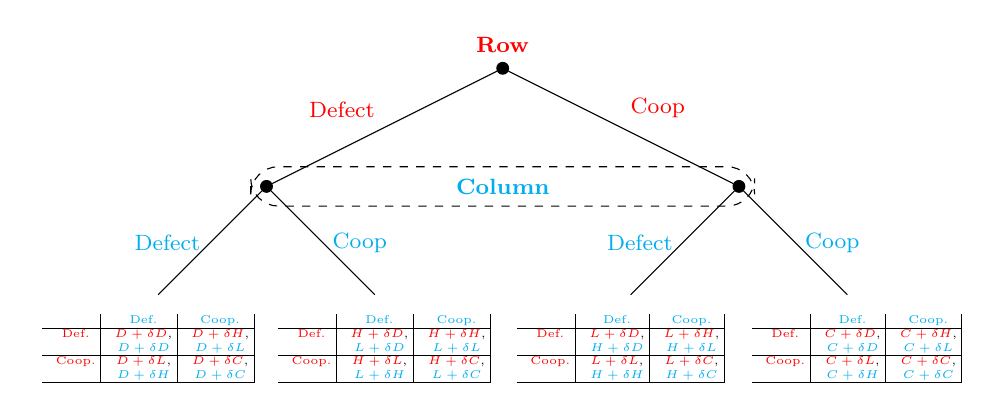
\begin{tikzpicture}[scale=1,font=\footnotesize]
    \tikzstyle{solid node}=[circle,draw,inner sep=1.5,fill=black]
    \tikzstyle{level 1}=[level distance=15mm,sibling distance=6cm]
    \tikzstyle{level 2}=[level distance=15mm,sibling distance=3cm]
    \node(0)[solid node,label=above:{\color{red} \textbf{Row}}]{}
      child{node(1)[solid node,label=above left:{}]{}
        child{node(3)[]{} edge from parent node[left]{\color{cyan}Defect}}
        child{node(4)[]{} edge from parent node[right]{\color{cyan}Coop}}
        edge from parent node[above left]{\color{red}Defect}
      }
      child{node(2)[solid node,label=above right:{}]{}
        child{node(5)[]{} edge from parent node[left]{\color{cyan}Defect}}
        child{node(6)[]{} edge from parent node[right]{\color{cyan}Coop}}
        edge from parent node[above right]{\color{red}Coop}
      };
    % info set
    \draw[dashed,rounded corners=10]($(1) + (-.2,.25)$)rectangle($(2) +(.2,-.25)$);
    \node at($(1)!.5!(2)$){\color{cyan} \textbf{Column}};
    % second stage
    \node[below] at(3){
      \tiny
      \scalebox{.82}{
      \begin{tabular}{*{3}{c<{\hspace{-4pt}}|}}
         & {\color{cyan} Def.} & {\color{cyan} Coop.} \\ \cline{1-3}
         {\color{red} Def.} & {\color{red} $D + \delta D$}, & {\color{red} $D + \delta H$},\\ 
                          & {\color{cyan}$D + \delta D$}  & {\color{cyan}$D + \delta L$} \\ \cline{1-3} 
         {\color{red} Coop.} & {\color{red} $D + \delta L$}, & {\color{red} $D + \delta C$},\\ 
                          & {\color{cyan}$D + \delta H$}  & {\color{cyan}$D + \delta C$} \\ \cline{1-3} 
      \end{tabular}
      }
    };
    \node[below] at(4){
      \tiny
      \scalebox{.82}{
      \begin{tabular}{*{3}{c<{\hspace{-4pt}}|}}
         & {\color{cyan} Def.} & {\color{cyan} Coop.} \\ \cline{1-3}
         {\color{red} Def.} & {\color{red} $H + \delta D$}, & {\color{red} $H + \delta H$},\\ 
                          & {\color{cyan}$L + \delta D$}  & {\color{cyan}$L + \delta L$} \\ \cline{1-3} 
         {\color{red} Coop.} & {\color{red} $H + \delta L$}, & {\color{red} $H + \delta C$},\\ 
                          & {\color{cyan}$L + \delta H$}  & {\color{cyan}$L + \delta C$} \\ \cline{1-3} 
      \end{tabular}
      }
    };
    \node[below] at(5){
      \tiny
      \scalebox{.82}{
      \begin{tabular}{*{3}{c<{\hspace{-4pt}}|}}
         & {\color{cyan} Def.} & {\color{cyan} Coop.} \\ \cline{1-3}
         {\color{red} Def.} & {\color{red} $L + \delta D$}, & {\color{red} $L + \delta H$},\\ 
                          & {\color{cyan}$H + \delta D$}  & {\color{cyan}$H + \delta L$} \\ \cline{1-3} 
         {\color{red} Coop.} & {\color{red} $L + \delta L$}, & {\color{red} $L + \delta C$},\\ 
                          & {\color{cyan}$H + \delta H$}  & {\color{cyan}$H + \delta C$} \\ \cline{1-3} 
      \end{tabular}
      }
    };
    \node[below] at(6){
      \tiny
      \scalebox{.82}{
      \begin{tabular}{*{3}{c<{\hspace{-4pt}}|}}
         & {\color{cyan} Def.} & {\color{cyan} Coop.} \\ \cline{1-3}
         {\color{red} Def.} & {\color{red} $C + \delta D$}, & {\color{red} $C + \delta H$},\\ 
                          & {\color{cyan}$C + \delta D$}  & {\color{cyan}$C + \delta L$} \\ \cline{1-3} 
         {\color{red} Coop.} & {\color{red} $C + \delta L$}, & {\color{red} $C + \delta C$},\\ 
                          & {\color{cyan}$C + \delta H$}  & {\color{cyan}$C + \delta C$} \\ \cline{1-3} 
      \end{tabular}
      }
    };
  \end{tikzpicture}
  \end{center} 
  Recall that $\delta$ is the subjective discount rate from stage to stage 
\end{frame}

\begin{frame}{Test Your Understanding}
  What should you do in the two-stage Prisoners' Dilemma 
  if your opponent plays \textit{Coop} in stage 1 and \textit{Coop} in stage 2?
  \begin{enumerate}[label=\textbf{\alph*)}]
    \item \textit{Coop} in stage 1, \textit{Coop} in stage 2
    \item \textit{Coop} in stage 1, \textit{Defect} in stage 2
    \item \textit{Defect} in stage 1, \textit{Coop} in stage 2
    \item \textit{Defect} in stage 1, \textit{Defect} in stage 2
  \end{enumerate}
\end{frame}

\begin{frame}{$\mathbb{T}$-stage repeated Prisoners' Dilemma}
  Suppose that $\mathbb{T}$ is a very large number, but we have played to the very last stage of a repeated Prisoners' Dilemma with that many stages:
  \begin{center}
    \begin{tabular}{*{4}{c|}}
      \multicolumn{2}{c}{} & \multicolumn{2}{c}{Column} \\ \cline{3-4}
      \multicolumn{1}{c}{} &        & Defect & Cooperate \\ \cline{2-4}
      \multirow{2}*{Row} & Defect   & Tot.$^R + D$, Tot.$^C + D$ & Tot.$^R + H$, Tot.$^C + L$ \\ \cline{2-4}
                         & Cooperate& Tot.$^R + L$, Tot.$^C + H$ & Tot.$^R + C$, Tot.$^C + C$ \\ \cline{2-4}
    \end{tabular} 
  \end{center}
  Let Tot.$^R$ and Tot.$^C$ represent the total payoffs that both players have earned over 
  stages 1 to $\mathbb{T} -1$
\end{frame}
